%\begin{noindent}
\begin{markdown}

# Hochspannungs-Gleichstrom-Übertragung (HGÜ)

\begin{figure}[H]
    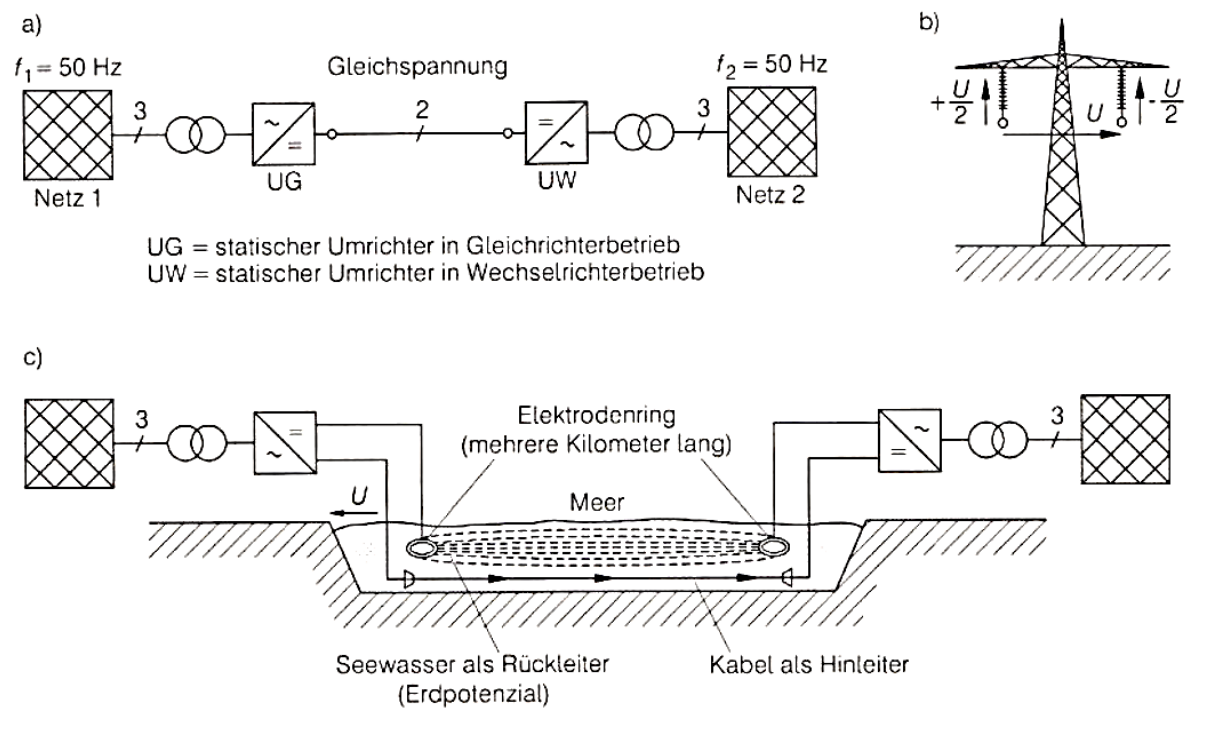
\includegraphics[width=\textwidth]{images/04-Hochspannungs-Gleichstrom-Ubertragung/Arten.png}
    \captionsetup{singlelinecheck=off}
    \caption[HGÜ Arten]{Arten von Hochspannungs-Gleichstrom-Übertragung
    \begin{enumerate}
        \item[a)] Prinzipielle Funktion
        \item[b)] Potentialverhältnisse an einer HGÜ-Freileitung
        \item[c)] HGÜ-Anlage für Seekabel
    \end{enumerate}
    }
\end{figure}

\vspace{1em}

**Vorteile**

- Weniger Übertragungsverluste _(Spannungsabfall wird nur durch ohmschen Widerstand bestimmt, Keine Wirbelstromverluste)_
- Mehr Energieübertragung _(Keine Blindleistungen, Keine Übertragung von Kurzschlussströmen)_
- Kann Störungen zwischen Drehstromnetzen verhindern.
- Kleinere Leiterquerschnitte
- Netzentkopplung _(Netze, die nicht synchron sind, können gekoppelt werden)_

\GrayBox{Ab ca. 600 km sind Freileitungen mit HGÜ-Technik wirtschaftlicher als mit Drehstromtechnik, bei Seekabeln bereits ab ca. 80 km.}

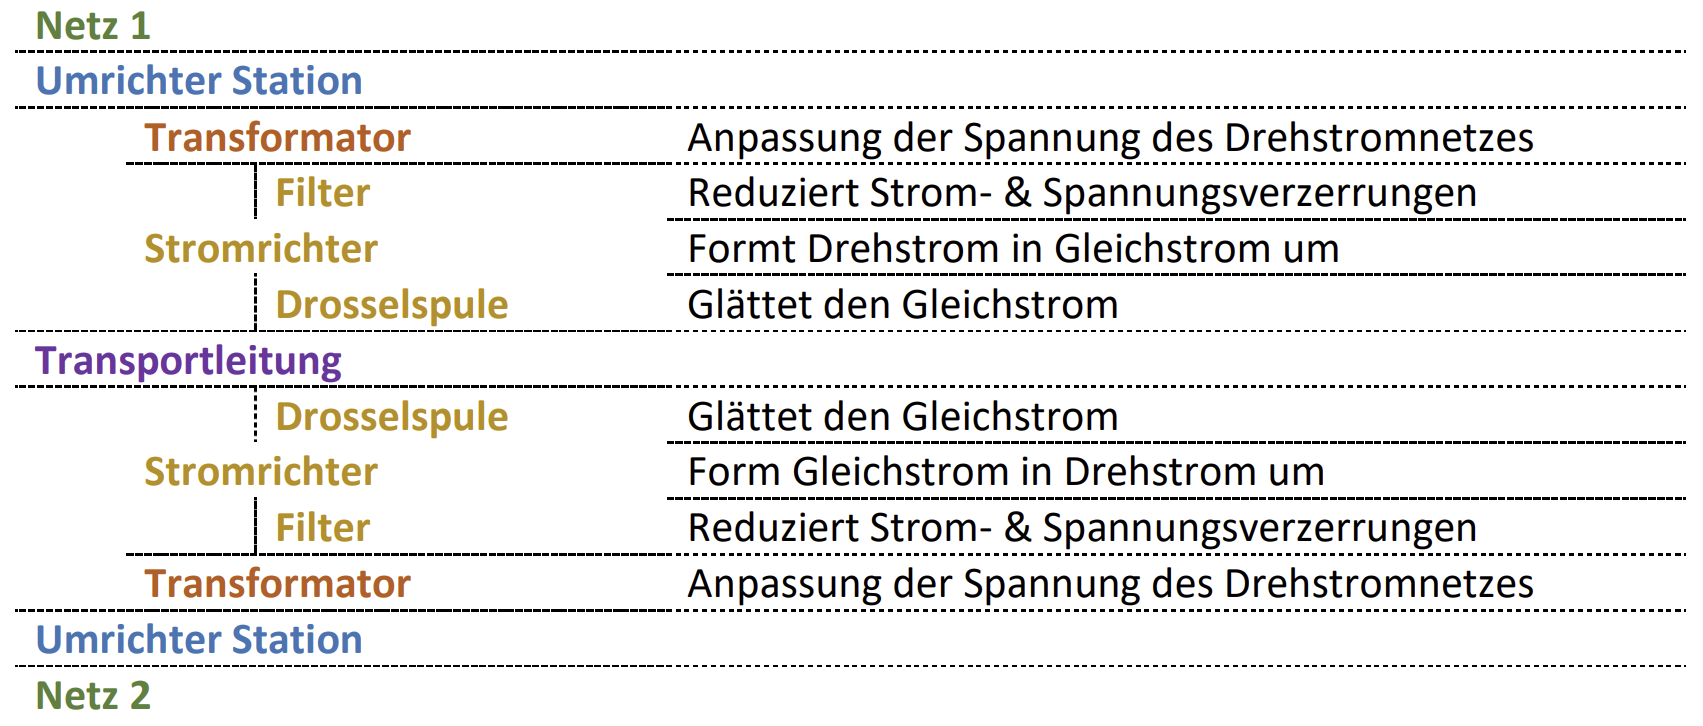
\includegraphics[width=\textwidth]{images/04-Hochspannungs-Gleichstrom-Ubertragung/Aufbau.png}

\end{markdown}